\documentclass[memoire.tex]{subfiles}

\chapter{Les architectures Big Data}

Une architecture Big Data est un regroupement d'outils permettant de gérer des données de leurs ingestion à leurs mise en valeur via des analyses.
Il faut savoir qu'il existe plusieurs architectures dans le domaine du Big Data, et qu'elles répondent à des besoins différents. Nous allons nous intéresser aux trois architectures les plus importantes, étant donné que les autres sont des dérivées des trois architectures principales. Avant de voir en détail ces trois architectures, nous allons voir de manière plus générale les différents composants qui peuvent se retrouver dans des architectures Big Data~\cite{ARCH_DATA}.
Les différents composants pouvant se retrouver dans une architecture Big Data sont illustrés sur la figure \ref{composants-architecture-big-data}.

\begin{figure}[!h]
	\centering 
	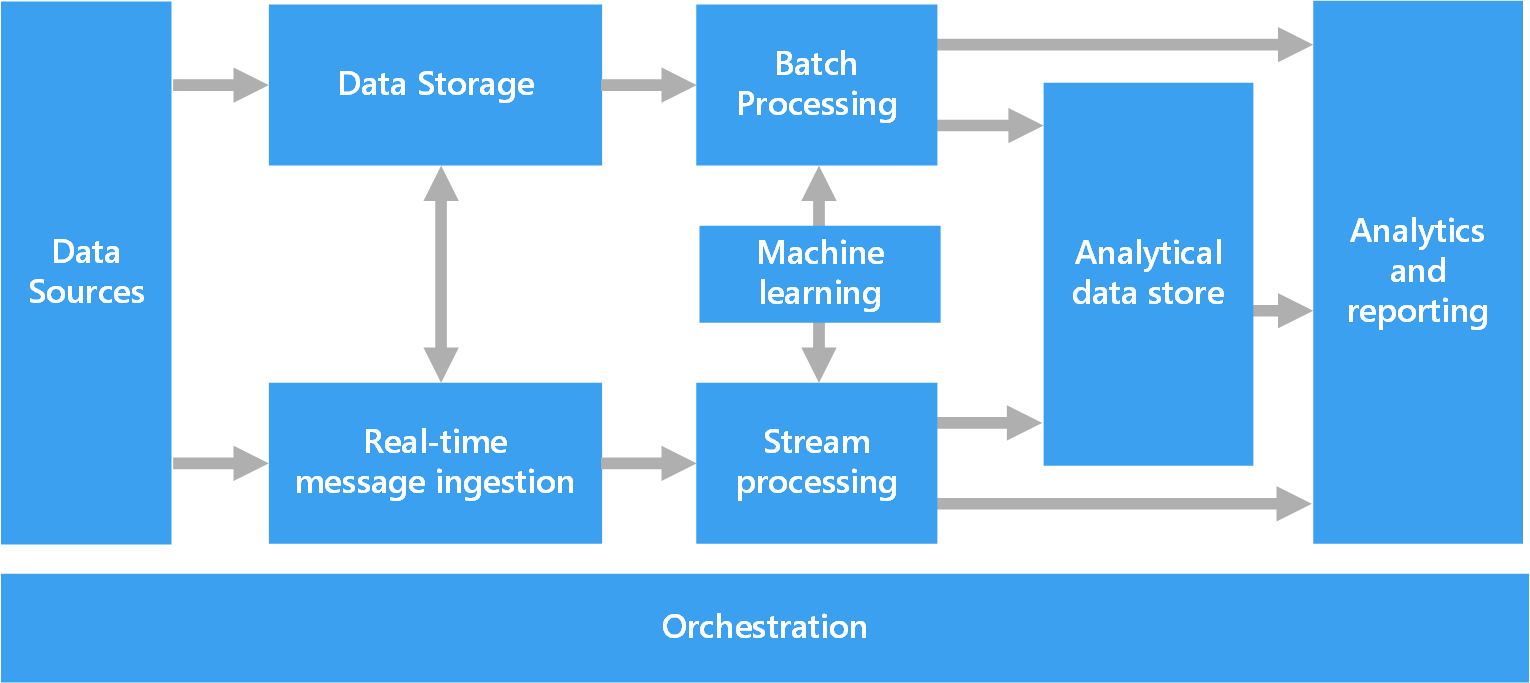
\includegraphics[scale=0.40]{img/big-data-comp.png}
	\caption{Composants d'une architecture Big Data}
	\label{composants-architecture-big-data}
\end{figure}

Nous allons maintenant détailler le rôle de chaque composant présenté dans le digramme ci dessus.

\begin{itemize}
\item \textbf{Source de données :} N'importe quelle solution Big Data a besoin d'une source de donnée en entrée. Voici quelques exemple de données qui peuvent être utilisée dans une architecture Big Data
\begin{itemize}
\item Des données issues de bases de données relationnelles.
\item Des fichiers statiques produits par des applications, des fichiers de logs par exemple.
\item Des sources de données en temps réel, par exemple des données de capteurs récupérés via des appareils IoTs.
\end{itemize}

\item \textbf{Stockage des données :} Une solution de stockage de données est indispensable dans le cas de traitement des données par lot ({\ref{a:traitement-donnees-batch}}), et peut s'avérer utile lors de traitements des données en temps réel ({\ref{a:traitement-donnees-real-time}}) si l'on souhaite conserver les données reçu en plus de les traiter. Le deuxième cas ou un stockage de donnée puet être utile pour le traitement en temps réel, est si l'on a besoin d'agréger des données statiques avec les données en temps réel. Ces solutions de stockage doivent être capable de gérer divers formats de données, et surtout ils doivent être distribués ({\ref{a:architecture-repartie}}).

\item \textbf{Traitement par lot ({\ref{a:traitement-donnees-batch}}) :} Les jeux de données étant trop lourd lors d'un traitement par lots, il est nécessaire de pouvoir exécuter une tâche de traitement de longue durée afin de filtrer, agréger et préparer les données en vue de leur analyse. En général, ce genre de traitement implique une lecture de fichier source et une écriture dans des nouveaux fichiers. Le traitement des données peut s'effectuer par des programmes java, scala ou Python ou encore via des outils spécialisé comme MapReduce ou Spark.  

\item \textbf{Ingestion de messages en temps réel : } Si la solution doit interagir avec des sources de données en temps réel, l'architecture doit impérativement implémenter un moyen de récupérer ces données et de les stocker temporairement dans une file d'attente afin de pouvoir les temporiser. Cela permet d'éviter la perte de données entrante, et permet d'envoyer les données à la solution de traitement quand elle est disponible et de ne pas la surcharger. Généralement on utilise des messages brokers pour ce genre de tâches.  

\item \textbf{Traitement de flux ({\ref{a:traitement-donnees-real-time}}) :} Une fois les données récupérées, elles doivent être filtrées, agrégées puis préparer pour l'analyse.

\item \textbf{Magasin de données analytique : } 

\item \textbf{Analyse, rapports et visualisation des données :} 

\item \textbf{Orchestration : } La majorité des solutions Big Data consistent a effectuer des traitements de données répétés, ayant pour but de transformer les données sources, les déplacer entre plusieurs endroits et les envoyer dans un magasin de données analytique ou bien les envoyer directement à un outil d'analyse.

\end{itemize}

\section{Architecture Data Lake}

\section{Architecture Lambda}

L'architecture Lambda a été crée dans le but de pouvoir à la fois traiter des données en batch et en streaming. Plus précisément, l'architecture lambda est composé de deux couches afin de gérer à la fois les batch et le streaming. Une couche est dédié pour traiter les données par batch, pour ensuite les rendre disponible (Ce qui est appelé une "view"). L'autre couche, s'occupe du streaming. Et à chaque donnée traitée, le résultat est mis à disposition. Grâce à ce fonctionnement lorsque l'on souhaite faire une requête, elle va pouvoir prendre en compte nos données récupérées par batch et par streaming.

\begin{figure}[!h]
	\centering 
	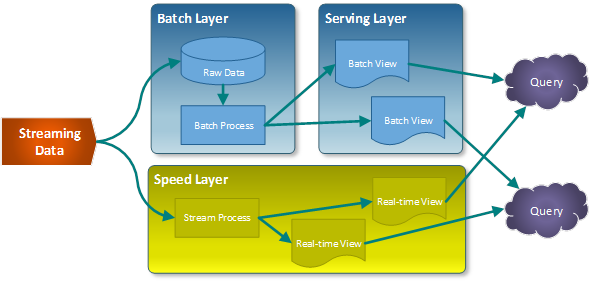
\includegraphics[scale=0.90]{img/lambda.png}
	\caption{Schéma de l'architecture Lambda}
	\label{Lambda}
\end{figure}

\section{Architecture Kappa}

L'architecture Kappa, se veut plus "simple". Le but étant de traiter toutes les données en streaming. Cela a pour conséquence de n'avoir qu'une seule couche contrairement aux deux nécessaire pour l'architecture Lambda. Mais cela ne permet pas de remplacer l'architecture Lambda, en effet il faut que les données que l'on récupère en Batch et la manière dont elles sont stockées, permettent de les traiter en streaming par la suite.

\begin{figure}[!h]
	\centering 
	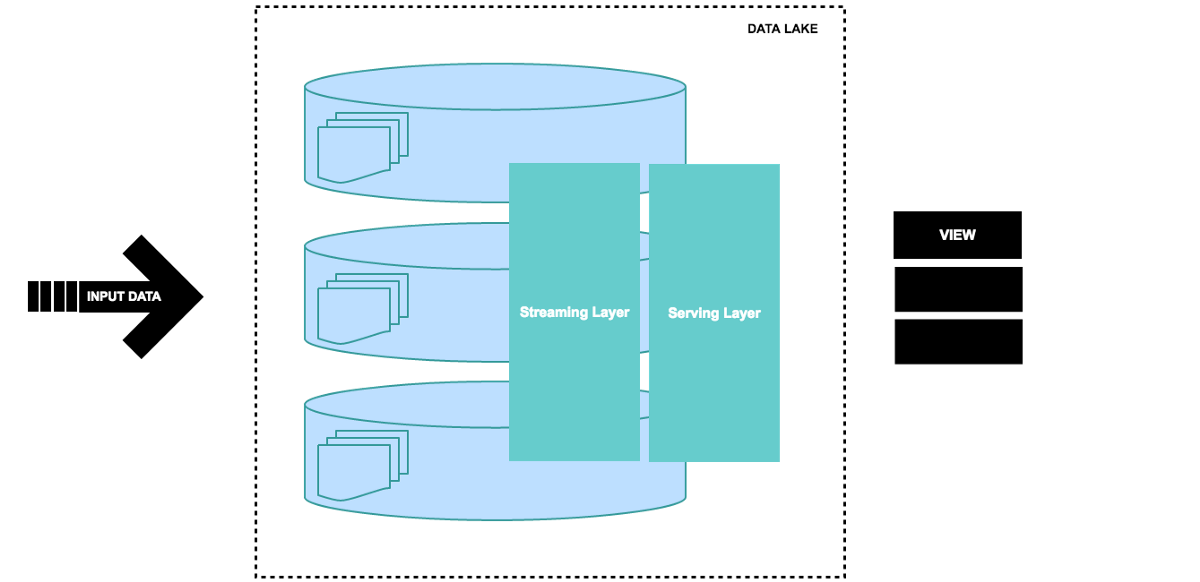
\includegraphics[scale=0.90]{img/kappa.png}
	\caption{Schéma de l'architecture Kappa}
	\label{Kappa}
\end{figure}